\documentclass[aps,floatfix,footinbib,superscriptaddress]{revtex4-1}
\usepackage{epsfig}
\usepackage{float}
\usepackage{epstopdf} %converting to PDF
\usepackage{braket}
\usepackage[utf8]{inputenc}
\usepackage{amsmath}
\usepackage{amssymb}
\usepackage{esint}
\usepackage{xcolor}
\usepackage{bbm}


\begin{document}
\title{Revealing the emergence of classicality in nitrogen-vacancy centers}

%Alt titles: 
%\title{Revealing the emergence of the classicality via NV center measurements}
%Revealing the emergence of the classical world via NV center measurements
%The emergence of a classical NV-center spin /via nuclear-spin decoherence
%The emergence of redundancy in nuclear spin environments of an NV center.
%Quantum Darwinism in action (in the lab): The emergence of redundancy in nuclear spin environments of an NV center.

\global\long\def\avg#1{\langle#1\rangle}

\global\long\def\p{\prime}

\global\long\def\dg{\dagger}

\global\long\def\ket#1{|#1\rangle}

\global\long\def\bra#1{\langle#1|}

\global\long\def\proj#1#2{|#1\rangle\langle#2|}

\global\long\def\inner#1#2{\langle#1|#2\rangle}

\global\long\def\tr{\mathrm{tr}}

\global\long\def\pd#1#2{\frac{\partial#1}{\partial#2}}

\global\long\def\spd#1#2{\frac{\partial^{2}#1}{\partial#2^{2}}}

\global\long\def\der#1#2{\frac{d#1}{d#2}}

\global\long\def\im{\imath}

\global\long\def\S{\mathcal{S}}

\global\long\def\A{\mathcal{A}}

\global\long\def\F{\mathcal{F}}

\global\long\def\E{\mathcal{E}}

\global\long\def\As{{^{\sharp}}\hspace{-1mm}\mathcal{A}}

\global\long\def\Fs{{^{\sharp}}\hspace{-0.7mm}\mathcal{F}}

\global\long\def\Es{{^{\sharp}}\hspace{-0.5mm}\mathcal{E}}

\global\long\def\EsG{{^{\sharp}}\hspace{-0.5mm}\mathcal{E}_{G}}

\global\long\def\EsB{{^{\sharp}}\hspace{-0.5mm}\mathcal{E}_{B}}

\global\long\def\FsG{{^{\sharp}}\hspace{-0.5mm}\F_{G}}

\global\long\def\FsB{{^{\sharp}}\hspace{-0.5mm}\F_{B}}

\global\long\def\Fd{{^{\sharp}}\hspace{-0.7mm}\mathcal{F}_{\delta}}

\global\long\def\EG{\mathcal{E}_{G}}

\global\long\def\EB{\mathcal{E}_{B}}

\global\long\def\O{\mathcal{O}}

\global\long\def\SgF{\S d\F}

\global\long\def\SgEF{\S d\left(\E/\F\right)}

\global\long\def\U{\mathcal{U}}

\global\long\def\V{\mathcal{V}}

\global\long\def\H{\mathbf{H}}

\global\long\def\SO{\Pi_{\S}}

\global\long\def\PO{\hat{\Pi}_{\S}}

\global\long\def\SSH{\tilde{\Pi}_{\S}}

\global\long\def\EO{\Upsilon_{k}}

\global\long\def\ESH{\Omega_{k}}

\global\long\def\HSF{\mathbf{H}_{\S\F}}

\global\long\def\HSEF{\mathbf{H}_{\S\E/\F}}

\global\long\def\HS{\mathbf{H}_{\S}}

\global\long\def\ES{H_{\S}(t)}

\global\long\def\ESo{H_{\S}(0)}

\global\long\def\EgF{H_{\SgF} (t)}

\global\long\def\EgE{H_{\S d\E}(t)}

\global\long\def\EgEF{H_{\SgEF} (t)}

\global\long\def\EF{H_{\F}(t)}

\global\long\def\EFo{H_{\F}(0)}

\global\long\def\ESF{H_{\S\F}(t)}

\global\long\def\ESEF{H_{\S\E/\F}(t)}

\global\long\def\ESSEF{H_{\tilde{\S}\S\E/\F}(t)}

\global\long\def\EEFo{H_{\E/\F}(0)}

\global\long\def\EEF{H_{\E/\F}(t)}

\global\long\def\HPB{H(\PB)}

\global\long\def\MI{I\left(\S:\F\right)}

\global\long\def\aMI{\left\langle \MI\right\rangle _{\Fs}}

\global\long\def\BS{\Pi_{\S} }

\global\long\def\PB{\hat{\Pi}_{\S} }

\global\long\def\QD{\mathcal{D}\left(\Pi_{\S}:\F\right)}
\global\long\def\QD{\mathcal{D}(\Pi_{\S}:\F)}

\global\long\def\QDp{\mathcal{D}\left(\PB:\F\right)}
\global\long\def\QDpIL{\mathcal{D}(\PB:\F)}

\global\long\def\JI{J\left(\Pi_{\S}:\F\right)}

\global\long\def\CI{H\left(\F\left|\Pi_{\S}\right.\right)}

\global\long\def\CIp{H\left(\F\left|\PB\right.\right)}

\global\long\def\CS{\rho_{\F\left|s\right.}}

\global\long\def\CSu{\tilde{\rho}_{\F\left|s\right.}}

\global\long\def\CSp{\rho_{\F\left|\hat{s}\right.}}

\global\long\def\CEF{H_{\F\left|s\right.}}

\global\long\def\CEFp{H_{\F\left|\hat{s}\right.}}

\global\long\def\psiz{\ket{\psi_{\E\left|0\right.\hspace{-0.4mm}}}}

\global\long\def\psio{\ket{\psi_{\E\left|1\right.\hspace{-0.4mm}}}}

\global\long\def\psiinner{\inner{\psi_{\E\left|0\right.\hspace{-0.4mm}}}{\psi_{\E\left|1\right.\hspace{-0.4mm}}}}

\global\long\def\QDz{\boldsymbol{\delta}\left(\S:\F\right)_{\left\{  \sigma_{\S}^{z}\right\}  }}

\global\long\def\NQD{\bar{\boldsymbol{\delta}}\left(\S:\F\right)_{\BS}}

\global\long\def\EFS{H_{\F\left| \BS\right. }(t)}

\global\long\def\EFSM{H_{\F\left| \left\{  \ket m\right\}  \right. }(t)}

\global\long\def\Hol{\chi\left(\Pi_{\S}:\F\right)}
\global\long\def\HolIL{\chi(\Pi_{\S}:\F)}

\global\long\def\Holp{\chi\left(\PB:\F\right)}
\global\long\def\HolpIL{\chi(\PB:\F)}

\global\long\def\ch{\raisebox{0.5ex}{\mbox{\ensuremath{\chi}}}_{\mathrm{Pointer}}}

\global\long\def\rhoS{\rho_{\S}(t)}

\global\long\def\rhoSo{\rho_{\S}(0)}

\global\long\def\rhoSF{\rho_{\S\F} (t)}

\global\long\def\rhoSgEF{\rho_{\SgEF} (t)}

\global\long\def\rhoSgF{\rho_{\SgF} (t)}

\global\long\def\rhoF{\rho_{\F}(t)}

\global\long\def\rhoFp{\rho_{\F}(\pi/2)}

\global\long\def\LE{\Lambda_{\E}(t)}

\global\long\def\LEc{\Lambda_{\E}^{\star}(t)}

\global\long\def\LEij{\Lambda_{\E}^{ij}(t)}

\global\long\def\LF{\Lambda_{\F}(t)}

\global\long\def\LFij{\Lambda_{\F}^{ij} (t)}

\global\long\def\LFc{\Lambda_{\F}^{\star}(t)}

\global\long\def\LEF{\Lambda_{\E/\F} (t)}

\global\long\def\LEFij{\Lambda_{\E/\F}^{ij}(t)}

\global\long\def\LEFc{\Lambda_{\E/\F}^{\star}(t)}

\global\long\def\Lkij{\Lambda_{k}^{ij}(t)}

\global\long\def\Hb{H}

\global\long\def\kE{\kappa_{\E}(t)}

\global\long\def\kEF{\kappa_{\E/\F}(t)}

\global\long\def\kF{\kappa_{\F}(t)}

\global\long\def\ts{t=\pi/2}

\global\long\def\QCB{\bar{\xi}_{QCB}}

\global\long\def\mc#1{\mathcal{#1}}

\global\long\def\MD{\lambda}

\global\long\def\up{\mathord{\uparrow}}

\global\long\def\down{\mathord{\downarrow}}

\global\long\def\Cku{\rho_{k\left|\up\right.}}

\global\long\def\Ckd{\rho_{k\left|\down\right.}}

\global\long\def\f{\mathcal{J}}

\global\long\def\onlinecite#1{\cite{#1}}

\newcommand{\todo}[1]{\textcolor{red}{#1}}

\title{Supplementary Information -- Revealing the emergence of classicality in nitrogen-vacancy centers}

\author{T. Unden}
\affiliation{Institute for Quantum Optics, Ulm University, Albert-Einstein-Allee 11, Ulm 89081, Germany}

\author{D. Louzon}
\affiliation{Institute for Quantum Optics, Ulm University, Albert-Einstein-Allee 11, Ulm 89081, Germany}
\affiliation{Racah Institute of Physics, The Hebrew University of Jerusalem, Jerusalem 91904, Israel}

\author{M. Zwolak}
\affiliation{Center for Nanoscale Science and Technology, National Institute of Standards and Technology, Gaithersburg,
Maryland 20899, U.S.A.}

\author{W. H. Zurek}
\affiliation{Theory Division, Los Alamos National Laboratory, Los Alamos, NM, 87545, U.S.A.}

\author{F. Jelezko}
\affiliation{Institute for Quantum Optics, Ulm University, Albert-Einstein-Allee 11, Ulm 89081, Germany}
\affiliation{Center for Integrated Quantum Science and Technology (IQ$^\text{{st}}$), Ulm University, 89081 Germany}

\maketitle

\renewcommand\thefigure{S\arabic{figure}}

\section{Experimental Setup and Control}

The diamond sample (IIa) is grown via Chemical Vapor Deposition (CVD). The isotopic composition is $98.9$ \% $^{12}C$. The concentration of carbon isotope nuclear spins ($1.1$ \% $^{13}$C) gives a significant probability to find multiple weakly coupled $^{13}$C in the frozen core of a NV center. Single NV center are introduced into the diamond from residual nitrogen in the CVD plasma.

For optical manipulation and detection of single NV centers in bulk diamond we use a home-built confocal microscope and for initialization and readout of the NV ground state spin green laser excitation ($532$ nm). An avalanche photodiode detects the corresponding fluorescence and a permanent magnet gives the static field ($\approx440$ G). We drive the electronic (NV) and nuclear ($^{13}$C) spin transitions via MW and RF fields via a thin copper wire close to the NV center and an arbitrary-wave form generator. The MW/RF phase gives the rotation axis of a pulse. We insert a $\frac{\pi}{2}$ phase-shift to get rotations around the $y$-axis. For manipulation, the typical Rabi frequencies are $40$ MHz for the electron spin rotations and $5$ kHz for nuclear spin rotations.

The DD sequence proposed in Ref.~\cite{Cas2015} provides control. Adjusting the timing $(\tau_1,\tau_2, \tau_3)$ and therefore the interpulse spacing $\tau$ can give an arbitrary filter-function for the DD sequence. We focus on the first harmonic and set the other contributions up to $4^{th}$ order to zero. The strength of the filter-function is set by the filter coefficients  $f_1=f_{DD},f_2=0,f_3=0,f_4=0$ and we solve the equations (see Ref.~\cite{Cas2015})
\begin{equation}
f_k = \frac{4}{\pi k} \left[\sum_{j=1}^{2} (-1)^j\left[(-1)^k-1\right]\sin\left(2\pi k \theta_j\right)+\sin\left(k\frac{\pi}{2}\right)\right]
\end{equation}
for $k=1-4$ numerically to get the corresponding pair of times 
\begin{align}
\tau_1 &= \frac{\theta_1}{\omega_{DD}}\\
\tau_2 &= \frac{\theta_2-\theta_1}{\omega_{DD}}\\  
\tau_3 &= \frac{1}{4\omega_{DD}}.
\end{align}
The frequency $\omega_{DD}=\frac{1}{2\tau}$ is the center of the control filter. Any effective coupling 
\begin{equation}
\frac{f_{DD}A_\perp}{2} \in \frac{1}{\pi}A_\perp\left(-8\cos(\frac{\pi}{9})+4,8\cos(\frac{\pi}{9})-4\right)
\end{equation}
is possible, where $A_\perp$ is the perpendicular HF coupling strength of an individual nuclear spin. 

In Fig.~\ref{fig:S1}, we show the coherent interaction between the electron and nuclear spin $\E_1$ for two different strengths of the filter-function. When the effective coupling increases from $\frac{0.1A_\perp}{2}$ to $\frac{0.2A_\perp}{2}$, the frequency of the oscillation doubles. Figure~\ref{fig:S2} shows the coherent interaction between the electron and nuclear spin $\E_1$ for a fixed AXY repetition number and increasing effective coupling for the cases $N=8,16,32$. A filter strength of about $\frac{0.2\cdot A_\perp}{2}$ was used. For a certain $N$, we fine-tune $f_{DD}$ to achieve two qubit $\pi/2$-rotations.

\begin{figure}[H]
\centerline{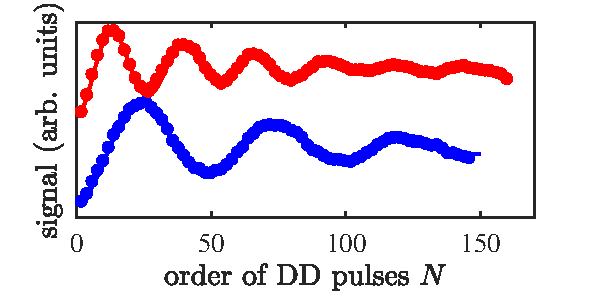
\psfig{file=figure/SFig1.pdf, width=0.5\linewidth}}
\caption{Electron spin coherence versus the DD pulse number when the pulse spacing is adjusted to the resonance of carbon spin 1. The entangling operation is via the AXY pulse sequence with filter coefficient $f_{DD}=0.1$ (blue) and doubled strength $f_{DD}=0.2$ (red). Solid lines are the result of a simulation, assuming dephasing and the measured hyperfine coupling strength (see Table 1). Errors are smaller than the data points.}
\label{fig:S1}
\end{figure}

\begin{figure}[H]
\centerline{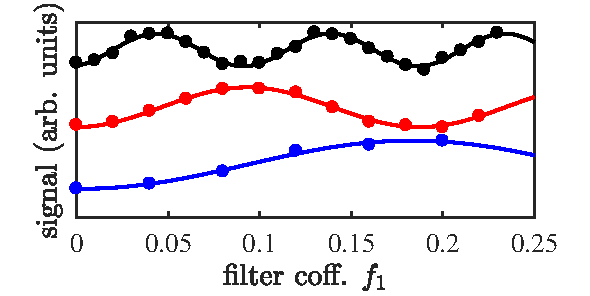
\psfig{file=figure/SFig2.pdf, width=0.5\linewidth}}
\caption{Electron spin coherence versus different filter strength. The entangling operation is via AXY-8 (blue)/16 (red)/32 (black). The solid lines are cosine fits (SSE from up to down of $4\cdot10^{-4}$, $6\cdot10^{-4}$ and $29\cdot10^{-4}$ ). Errors are smaller than the data points.}
\label{fig:S2}
\end{figure}

For further control, nuclear spin initialization and individual measurement via optical readout of the NV electronic spin is necessary. We achieve both by using an entangling gate mediated by $H^k$ (see main text), in combination with an asymmetric version~\cite{Souza4748} of it, to implement an iSwap gate ($e^{i\frac{\pi}{2}\sigma_xI_x}e^{i\frac{\pi}{2}\sigma_yI_y}$)~\cite{Cas17}. For the strongest coupled nuclear spin, it takes about $50\mu s$ to perform a swap operation, and for the weakest coupled one about $80\mu s$. We implement the entangling gate $R=e^{iH^k\frac{\pi}{2}}$ for each nuclear spin by carefully adjusting the repetition $N$ of the AXY sequence and the interpulse spacing $\tau$. To observe for example the nuclear Rabi oscillations shown in the main text, first the electron spin was optically polarized, then polarization was swapped to nuclear spin 1 with additional reinitialization of electron spin, application of the RF pulse follows and nuclear spin information is optically read out after a second iSwap gate. A typical gate fidelity of an iSwap gate is on the order of $0.8$ and is mainly limited by the electron coherence time of about 0.7 ms. Specific HF coupling values of the four nuclear spin system can be found in section \ref{sec.hf}. 

\section{Analysis}

The Holevo information requires the diagonal (in the $\PB$ basis of the system) component of the $\S\E$ density matrix. We thus can take the density matrix to be of the form $\rho_{\S\E}= p_{\up} \proj{\up}{\up} \otimes \rho_{\E\left|\up\right.} + p_{\down} \proj{\down}{\down} \otimes \rho_{\E\left|\down\right.}$, where the off-diagonal components in $\PB$ are not present (e.g., $\proj{\up}{\down}$ and $\proj{\down}{\up}$) and $\rho_{\E\left|\hat{s}\right.}=\bigotimes_k \rho_{\E_k\left|\hat{s}\right.}$ are the conditional nuclear density matrices in the corresponding electronic spin (pointer) sublevel $\hat{s}$. We determine the parameters of the nuclear density matrices (see for example section \ref{sec.GHZ}) by fitting the experimental data with simulation (and $p_{\up} = p_{\down} = 1/2$). The Lindbladian for the simulation consists of the coherent HF interaction and a pure dephasing term associated with the HF coupling to additional, weakly coupled nuclear spins. We precisely measure in advance the parallel and perpendicular components of the HF coupling to the four core spins and the dephasing rate. By performing this fitting, we correct the $\S\E$ density matrix for errors occurring during the tomography process. To correct also the impact of imperfect nuclear spin initialization, the individual nuclear spin density matrices are normalized, to take on the form 
\begin{equation}
\rho_{\E_k} = \begin{pmatrix}
\rho_{11} & \rho_{12}/P_k\\
\rho_{21}/P_k & \rho_{22}
\end{pmatrix} ,
\end{equation}
where $P_k$ is the initial degree of nuclear spin polarization (after the swap operations). This normalizes the experimental data to the optical contrast of NV Rabi oscillations. 

\section{Hyperfine coupling strength}\label{sec.hf}

Table~\ref{tab:HF} shows the hyperfine coupling strength of the different nuclei. The parallel component is estimated by analysis of AXY spectra and the perpendicular component by analyzing oscillations (see Fig.~\ref{fig:S1}) caused by resonant interaction when the interaction time is increased. 

\begin{table}[H]
\caption{Hyperfine interaction strength of the register.}
\begin{center}
\begin{tabular}{ c c c }
  \hline
  \textbf{nuc. spin} & \textbf{$\frac{A_\parallel}{2\pi}$ (kHz)} & \textbf{$\left| \frac{A_\perp}{2\pi}\right|$ (kHz)} \\ 
  \hline
  1 & $\phantom{-}93.5$ & $45.8$ \\
  2 & $\phantom{-}49.5$ & $35.3$ \\
  3 & $-26.3$ &$22.0$\\
  4 & $-47.1$ & $42.5$\\
  \hline
\end{tabular}
\end{center}
\label{tab:HF}
\end{table}

\section{Creation of an electronic-nuclear GHZ state}\label{sec.GHZ}

\begin{figure}[H]
\centerline{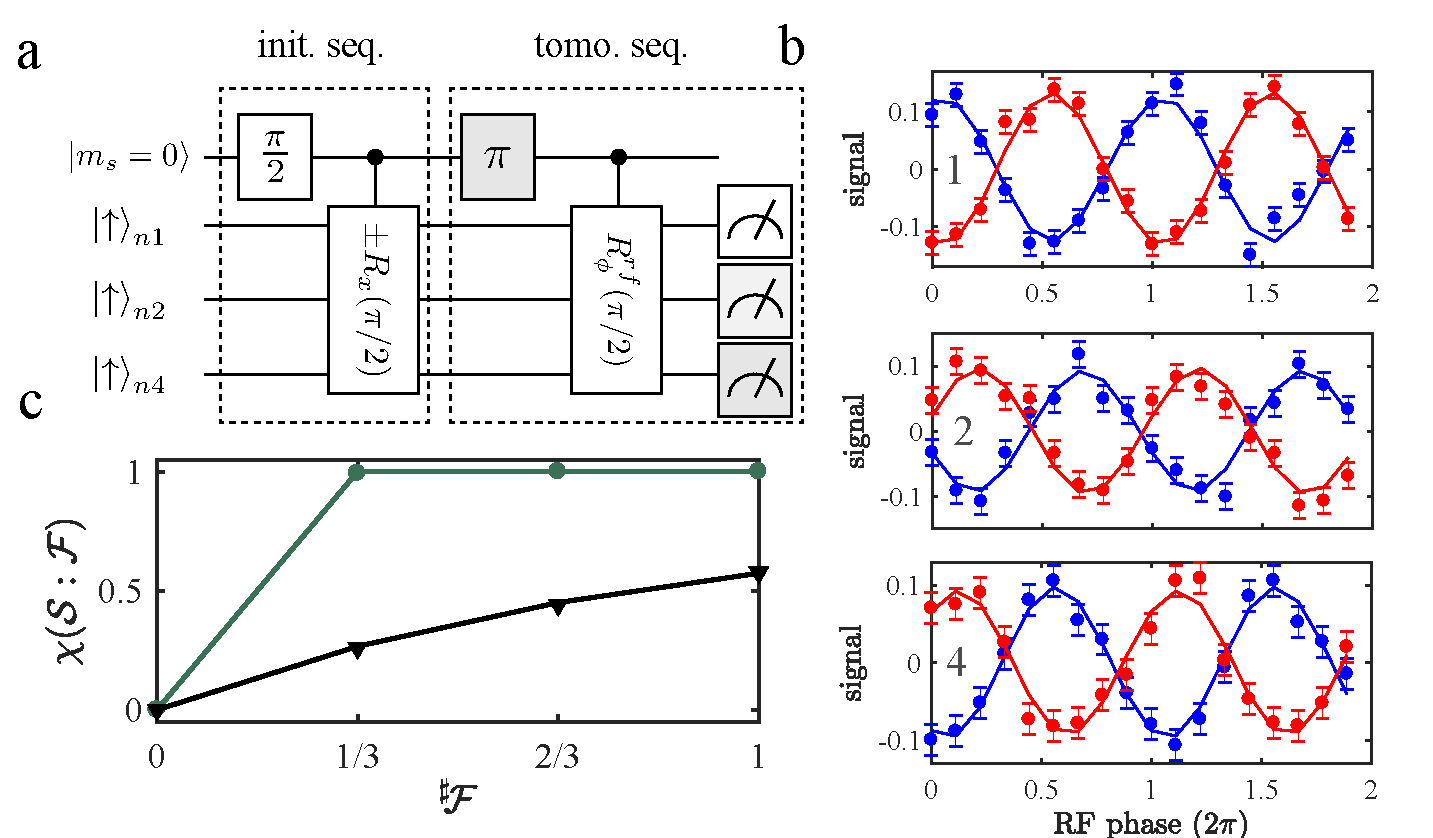
\psfig{file=figure/fig3.pdf, width=0.8\linewidth}}
\caption{Storing the central spin state redundantly in a three nuclear spin environment. (a) Protocol for creation and readout of the redundant state. The NV spin is first initialized and its polarization swapped to each individual nuclear spin by a repetitive process (not shown). An electronic superposition is then created by a $\frac{\pi}{2}$-pulse. Electronic-nuclear spin entanglement is created by a $\frac{\pi}{2}$ nuclear rotation in a direction conditional on the electronic spin state (see main text). Single nuclear spin tomography in the electronic subspace $\ket{m_s=-1}$ is performed by a selective $\frac{\pi}{2}$-pulse mediated by weak, resonant RF pulse. In addition, multiple measurements are performed with a different RF pulse phase $\phi$ to determine the phase of the nuclear spin superposition. An optional $\pi$-pulse in front of the last RF pulses can be applied for nuclear spin tomography in the electronic $\ket{m_s=0}$ subspace. The state of a single nuclear spin is in the end swapped to the NV spin and an optical readout follows. In a single sequence run, a nuclear spin is readout in one of the electronic subspaces. (b) Measurement results corresponding to the sequence shown in (a). The normalized NV fluorescence for each nuclear spin $(1,2,4)$ is presented. Tomography in the $\ket{m_s=0}$ ($\ket{m_s=-1}$) subspace is indicated in blue (red). Solid curves are results of a simulation (see Methods). Error bars represent one standard deviation of the measured data points. (c) Holevo information $\HolpIL$ based on the analysis of the data in (b) when different environment fraction sizes $\Fs$ are taken. The black data is corrected for error happening during tomography step (see the Analysis section) and the dark green data is also corrected for imperfect initial polarization. The solid curves show the result of a simulation considering the entangled state, $\ket{\up}_\S \otimes \ket{+}+\ket{\down}_\S \otimes \ket{-}$, with introduced initial polarization imperfections (black) and without (dark green). Errors are smaller than the data points.} 
\label{fig:3}
\end{figure}

The protocol to create a GHZ state is in Fig.~\ref{fig:3}a. For this demonstration, the three strongest coupled nuclear spins are chosen. We polarize the nuclear spins by first polarizing the electron spin via optical pumping and then swapping the electron polarization to each nuclear spin. This is followed by an electronic $\pi/2$-pulse and entanglement is sequentially created by the application of the entangling gate described in the main text. To observe correlations with a single nuclear spin, we utilize a selective RF $\pi/2$-pulse with variable phase $\phi$ ($R^{rf}_\phi$), which only rotates a single nuclear spin when the NV center is in the $m_s = -1$ state. To have access to the $m_s=0$ state, an optional MW $\pi$-pulse can be applied in front of the RF pulse. The results are shown in Fig.~\ref{fig:3}b for each nuclear spin. By varying the phase of the RF pulse, oscillations occur. For all nuclear spins we observe a $\pi$-phase shift between the data observed in the $m_s = 0$ (in blue) and $m_s = -1$ (in red) state, which indicates the orthogonal preparation of the state . The phase shift between signals of different nuclear spins is due to a different HF tensor with respect to the laboratory frame, defined by the RF-field axis~\cite{Laraoui15}. Here we focus mainly on classical correlations, but the result of an echo kind of sequence shows also the presence of quantum correlations in form of multiple quantum coherences~\cite{Baum85,Gaerttner17}, see next section.  

Figure~\ref{fig:3}c presents the Holevo information versus the fraction of nuclear spins in the fragment. In black we show the analyzed data, when error happening during the tomography sequence are corrected and in dark green the results when also error due to imperfect initial nuclear spin polarization is corrected (details are in the Analysis section). The typical degree of polarization is on the order of $(75\pm 5) \%$ for each nuclear spin and the fidelity for creating the GHZ state is about $40$ \% (see next section). Focusing on the data set shown in green, as soon as just one spin from the environment is intercepted, the Holevo information is already 1 bit. That is, access to a single environment spin already gives the pointer state of the system. Interception of further spins does not increase the Holevo information but only confirms the information from the first. This plateau -- the classical plateau -- signifies the appearance of redundant information. When error due to imperfect initial polarization are not corrected (black data), only the initial rise to the plateau is seen. Due to a non-zero initial entropy, the amount of information a single nuclear spin can store decreases and even when all environmental spins are taken into account, only about half a bit of central spin information can be intercepted. In general this is not true when a larger spin environment is considered~\cite{Zwolak09,Zwolak10-1}. 

\section{Multiple quantum coherence}

In Fig.~\ref{fig:S4}a, we show our sequence for testing quantum correlations after creating the redundant GHZ state. It is based on a Loschmidt echo, where the echo is perturbed by a free evolution period in between both entangling gates ($\pm R_x(\frac{\pi}{2})$). By increasing the free evolution period $\tau$, oscillations, Fig.~\ref{fig:S4}b, get visible, which can be attributed to the Larmor precession (about $0.5$ MHz) of the three nuclear spins and the sum of all Larmor frequencies (about $1.5$ MHz), which is a hint for multiple quantum coherences. The free evolution period was composed of a CPMG sequence, where the pulse spacing did not match to nuclear spin transitions. The reconstructed density matrix (shown in Fig.~\ref{fig:S4}c) is the result of a comparison of experimental data with simulated data (that takes only the diagonal and outer off-diagonal entries of the density matrix into account) and yields a state fidelity of $40$ \% with respect to a fully entangled GHZ state. 

\begin{figure}[H]
\centerline{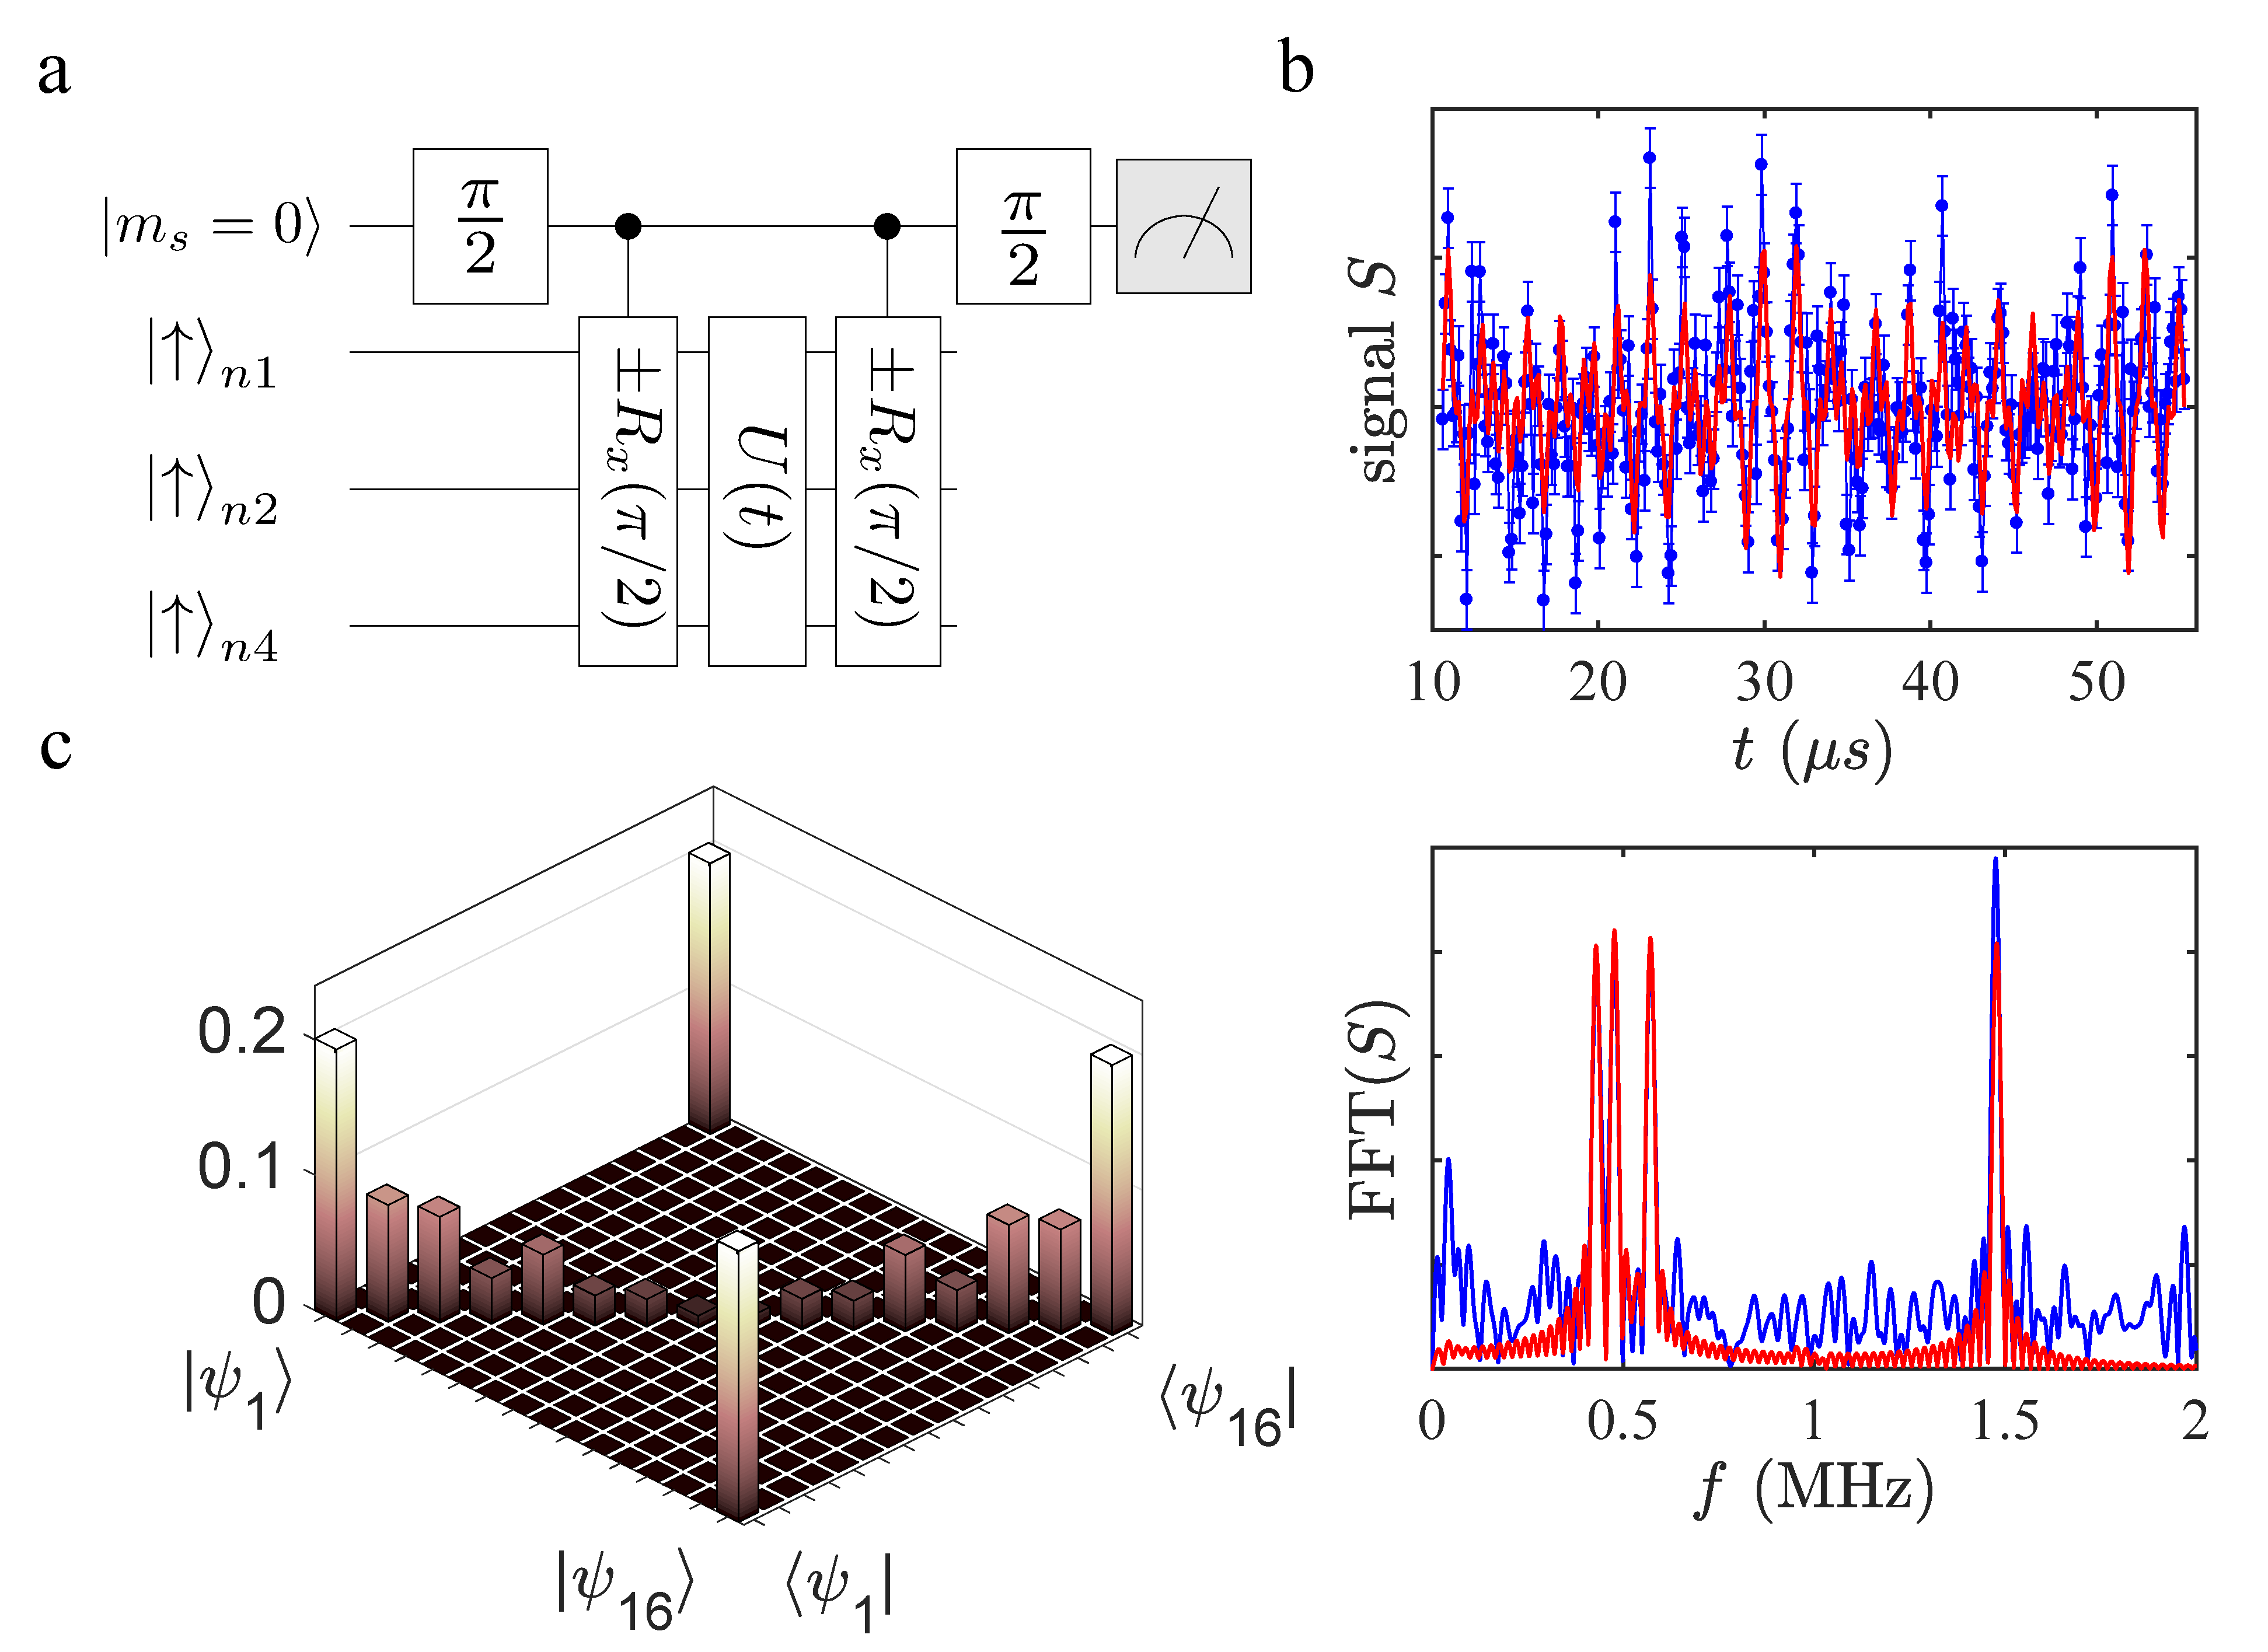
\psfig{file=figure/SFig4.pdf, width=0.6\linewidth}}
\caption{Results of the Loschmidt echo. (a) Sequence for testing multiple coherences present in the system. (b) Measurement (blue) and simulation (red) results with corresponding Fast Fourier Transform (FFT). Single Larmor frequency at a magnetic field of about $440G\approx 0.5 MHz$ is visible. The shift of each nuclear spin precession is due hyperfine interaction. Also visible is the sum of individual Larmor frequencies, which indicate multiple coherences present in the system. Error bars represent one standard deviation. (c) Reconstructed density matrix. with $\ket{\psi_1}=\ket{\uparrow}\ket{+}\ket{+}\ket{+}\ket{+}$ and  $\ket{\psi_{16}}=\ket{\downarrow}\ket{-}\ket{-}\ket{-}\ket{-}$.}
\label{fig:S4}
\end{figure}

\section{Chernoff Information}

In Fig.~\ref{fig:S5}, we show the quantum Chernoff information~\cite{Audenaert07} averaged over the four nuclear spins~\cite{Zwolak14,zwolak16}, i.e., the typical quantum Chernoff information $\QCB$, which sets an upper bound for redundancy rate in the asymptotic (large fragment size) limit. The redundancy is given by $\QCB \Es / \ln 1/\delta$, where $\Es$ is the total number of components in the environment. This equation requires sufficiently precise information (i.e., a small information deficit $\delta$) in order for the asymptotic limit to be accurate, otherwise the redundancy would be incorrectly given a value greater than $\Es$. 

\begin{figure}[H]
\centerline{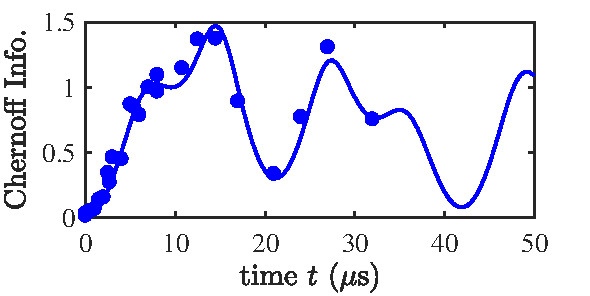
\psfig{file=figure/SFig5.pdf, width=0.5\linewidth}}
\caption{Chernoff Information. Solid line corresponds to a simulation based on the measured hyperfine interactions. Errors are smaller than the data points.}
\label{fig:S5}
\end{figure}

\section{NV Ramsey}

\begin{figure}[H]
\centerline{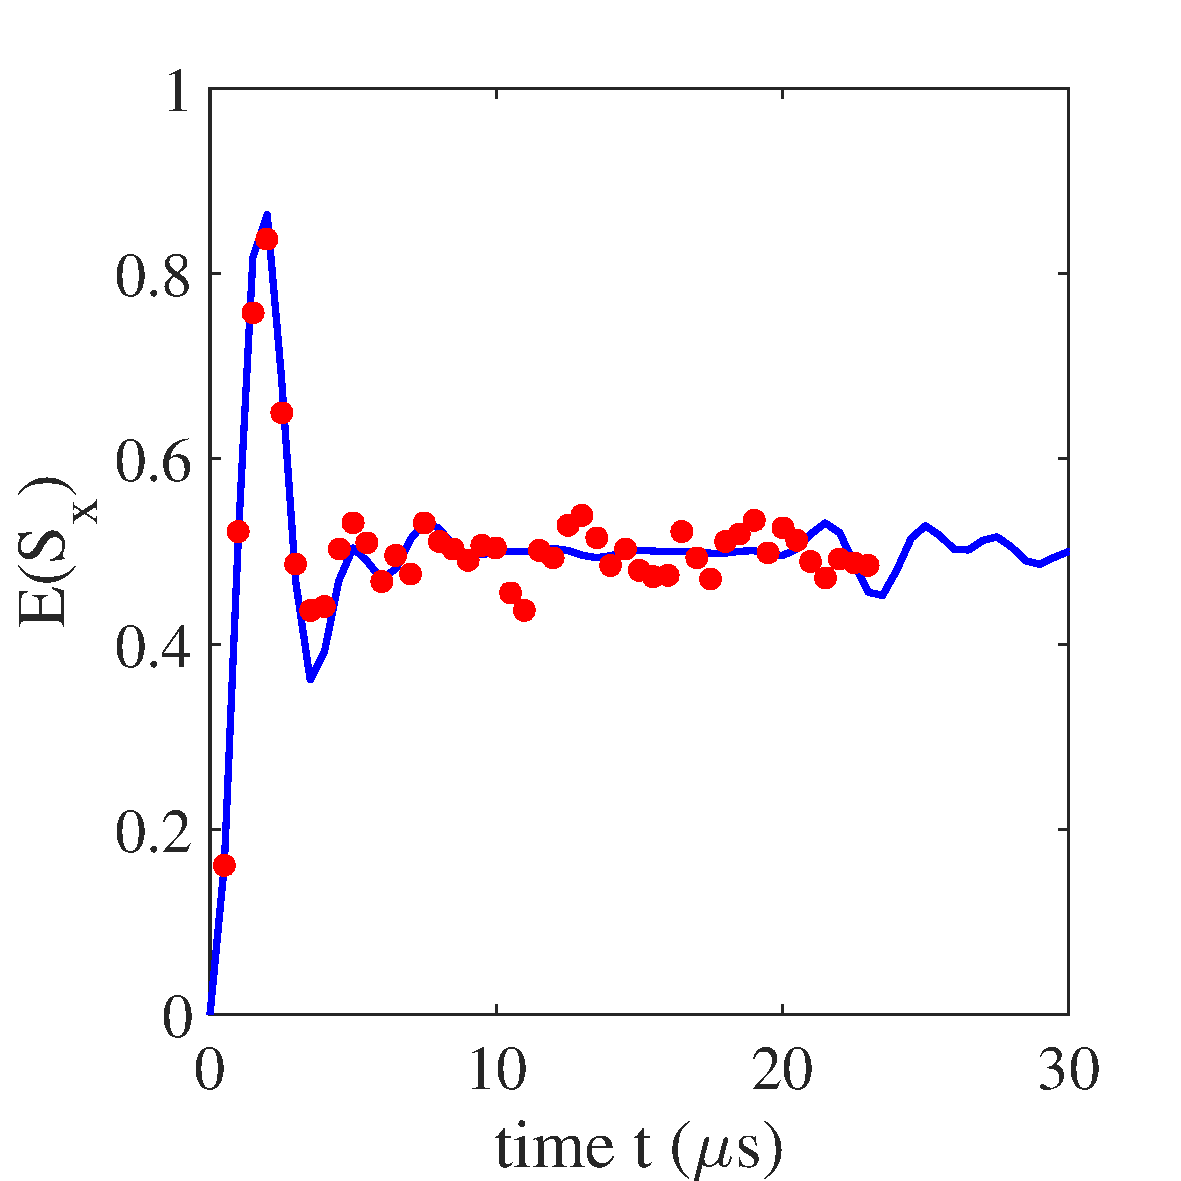
\psfig{file=figure/SFig3.pdf, width=0.35\linewidth}}
\caption{NV Ramsay experiment when the nuclear spin register is polarized to the $\ket{+}$ state. Solid line corresponds to a simulation based on the measured hyperfine interactions. Errors are smaller than the data points.}
\label{fig:S3}
\end{figure}

A Ramsay ($\frac{\pi}{2}$-pulse - wait $\tau$ - $\frac{\pi}{2}$-pulse) experiment performed on the electronic spin of NV center is shown in Fig.~\ref{fig:S3}. The four strongest coupled nuclear spins are polarized into the $\ket{+}$-state in this measurement. The initial state is therefore in accordance with the initial state of the experiment shown in the main text. 

\section{Potential redundancy in $^{13}C$ enriched diamonds}

Based on recently published hyperfine data of a 510 nuclear spin cluster~\cite{Nizovtsev18}, we show in Fig.~\ref{fig:S6} the number of central spin records over interaction time. The amount of information is estimated using quantum Chernoff information~\cite{Zwolak14,zwolak16}. The results are averaged over ten different realizations of the specified settings. In a highly concentrated $^{13}C$-diamond, a large amount (hundreds) of central spin records could be observed within a timescale of $\mu s$ when the initial nuclear spin polarization is large. At  high $^{13}C$ concentration unwanted  interaction (here in our analysis neglected) between nuclear spins will appear, but our current results show, that on the timescale ($\approx \mu s$) where redundancy increases, these interactions ($\approx$ Hz - kHz) can be neglected for a moderate $^{13}C$ enrichment and a high initial nuclear spin polarization.

\begin{figure}[H]
\centerline{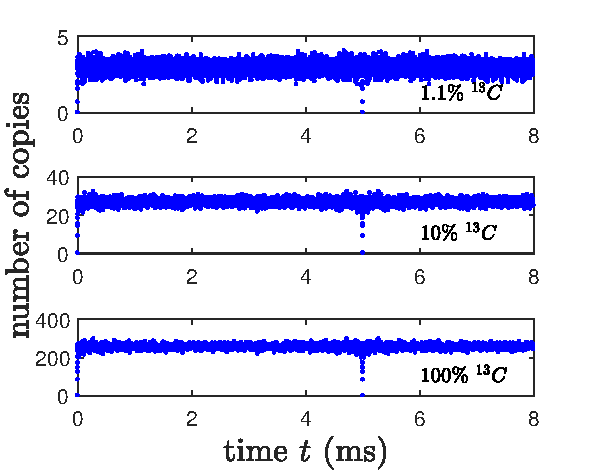
\psfig{file=figure/SFig6.pdf, width=0.5\linewidth}}
\caption{Number of copies of information versus the interaction time for various $^{13}C$ concentrations.}
\label{fig:S6}
\end{figure}

\bibliographystyle{apsrev}
\bibliography{reference}

\end{document}



